\documentclass{article}
\usepackage[utf8x]{inputenc}
\usepackage[colorlinks=true,linkcolor=black,citecolor=black,pdfusetitle,pagebackref=false]{hyperref}
\usepackage[nonumberlist,nohypertypes={glossary}]{glossaries}
\usepackage{graphicx}
\usepackage{multicol}
\usepackage[font=small,labelfont=bf]{caption}
\usepackage{subcaption}
\usepackage{authblk}
\usepackage{amsmath}
\usepackage{bm}
\usepackage[margin=1.5cm]{geometry}
\usepackage{cite}
\usepackage[usenames,dvipsnames,svgnames,table]{xcolor}
\usepackage{bigints}
\usepackage[normalem]{ulem}
\usepackage{mathrsfs}


\newenvironment{Figure}
  {\par\medskip\noindent\minipage{\linewidth}}
  {\endminipage\par\medskip}

\bibliographystyle{unsrt}
\renewcommand\refname{References}

\newacronym{cdi}
    {CDI}{coherent diffractive imaging}

\newacronym{odt}
    {ODT}{optical dipole trap}

\newacronym{bec}
    {BEC}{Bose-Einstein condensate}

\newacronym{fort}
    {FORT}{far-off-resonance trap}

\newacronym{ta}
    {TA}{tapered amplifier}

\newacronym{caes}
    {CAES}{cold-atom electron source}

\newacronym{xfel}
    {XFEL}{x-ray free electron laser}

\newacronym{mot}
    {MOT}{magneto-optical trap}

\newacronym{ecdl}
    {ECDL}{external cavity diode laser}

\newacronym{aom}
    {AOM}{acousto-optical modulator}

\newacronym{slm}
    {SLM}{spatial light modulator}

\newacronym{mopa}
    {MOPA}{master-oscillator power amplifier}

\newacronym{na}
    {NA}{numerical aperture}

\newacronym{ar}
    {AR}{anti-reflection}

\newacronym{ccd}
    {CCD}{charge-coupled device}

\newacronym{cro}
    {CRO}{cathode ray oscilloscope}

\newacronym{pbs}
    {PBS}{polarising beam splitter}

\newacronym{bs}
    {BS}{beam splitter}

\newacronym{npbs}
    {NPBS}{non-polarising beam splitter}

\newacronym{tec}
    {TEC}{thermo-electric cooler}

\newacronym{cw}
    {CW}{continuous wave}

\newacronym{mcp}
    {MCP}{microchannel plate}

\newacronym{fwhm}
    {FWHM}{full-width half maximum}

\newacronym{pdh}
    {PDH}{Pound-Drever-Hall}
    
\newacronym{ps}
    {PS}{polarisation spectroscopy}
    
\newacronym{obe}
    {OBE}{optical Bloch equation}
    
\newacronym{davll}
    {DAVLL}{dichroic atomic vapour laser lock}

\newacronym{mts}
    {MTS}{modulation transfer spectroscopy}

\newacronym{snr}
    {SNR}{signal-to-noise ratio}

\newacronym{lsd}
    {LSP}{linear spectral density}


\makeglossaries

\begin{document}
\title{Sub-kilohertz linewidth lasers using polarization spectroscopy}
\author[1]{J. S. J. Torrance}
\author[1]{B. M. Sparkes}
\author[1]{R. E. Scholten}

\affil[1]{School of Physics, The University of Melbourne, Victoria 3010 Australia}

\maketitle

\begin{abstract}
Polarization spectroscopy is a laser frequency stabilization technique that probes the wavelength dependent birefringence induced in an atomic medium by a circularly polarized pump laser beam. The signal dependson refractive index rather than absorption and the bandwidth is therefore not limited by the transition lifetime unlike other common techniques such as saturated absorption spectroscopy. Polarization spectroscopy has been shown to offer high bandwidth locking to an atomic reference, and linewidth narrowing, without requiring radio-frequency electronics. We investigate the noise-limited bandwidth and demonstrate sub-kHz laser linewidths using two conventional \glspl*{ecdl} and a heterodyne measurement.
\end{abstract}

\begin{multicols}{2}

\section{Intro}
Laser frequency stabilization to atomic references is essential to numerous applications including the cooling and trapping of atoms\cite{uetake_high_2008, ye_stable_2010, akamatsu_narrow_2012} and high resolution spectroscopy\cite{rafac_sub-dekahertz_2000}. In addition to stabilizing the frequency, narrowing the spectral linewidth of lasers is important to applications such as atomic clocks\cite{ludlow_sr_2008} and metrology\cite{metcalf_laser_1999, ye_quantum_2008, demtroder_laser_2003}.

There are a number of desirable traits in laser frequency stabilization schemes such as being able to stabilize to an atomic reference, being free of frequency and amplitude modulation, having high bandwidth in order to achieve low spectral linewidths, simplicity of implementation and low cost.

Common techniques for stabilization range from saturated absorption spectroscopy, which can achieve diode laser linewidths in the region of 150\,kHz\cite{cuneo_optically_1994}, to elaborate experiments involving extremely high finesse optical cavities that are able to achieve sub-Hertz linewidths using the \gls*{pdh} technique\cite{ludlow_compact_2007}.

The ability to stabilize a laser's frequency to an atomic reference, rather than to an arbitrary frequency, is frequently essential to experiments. Techniques such as saturated absorption spectroscopy\cite{maguire_theoretical_2006, haroche_theory_1972, preston_doppler-free_1996}, \gls*{davll}\cite{corwin_frequency-stabilized_1998,millett-sikking_davll_2007}, \gls*{mts}\cite{shirley_modulation_1982, mccarron_modulation_2008,xiang-hui_ultra-stable_2009} and Sagnac interferometry\cite{robins_Interferometric_2002,jundt_non-linear_2003} lock to atomic references whereas optical cavity techniques such as \gls*{pdh}\cite{drever_laser_1983} require a secondary lock to maintain absolute frequency stability. \Gls*{ps} is another technique that stabilizes a laser's frequency to an atomic transition by probing induced birefringence in an atomic sample, avoiding the need for frequency modultation.

Frequency modulation of the laser is required for some locking techniques but it can interfere with experimental applications so it is often desirable to avoid direct modulation of the laser's frequency using techniques such as \gls*{ps} or \gls*{davll} or by modulating only one beam from the laser using an \gls*{aom} or similar. This can be achieved with techniques that do not require modulation or by modulation of only the beam used in the locking setup using \glspl*{aom} or similar. \Gls*{ps} is a technique that requires no modulation.

Some locking techniques are limited by the evolution of the atomic states which evolve slower than the lifetime of the excited state (26.2\,ns for Rb$^{85}$). Unlike these techniques \gls*{ps} is not limited by the rates at which the atomic populations evolve. At high frequency \Gls*{ps} depends on interactions with the refractive index of the atomic medium and is thus technically and noise limited.

It has been shown previously that \gls*{ps} can be used to reduce the linewidth of a distributed feedback diode from 2\,MHz to 20\,kHz\cite{torii_laser-phase_2012} and of diode lasers to 65\,kHz\cite{yoshikawa_frequency_2003}. In this letter we utilize high bandwidth feedback to the laser diode to achieve linewidths of order 1\,kHz.

\section{Pol Spec Theory}

\begin{Figure}
    \centering
    \captionsetup{type=figure}
    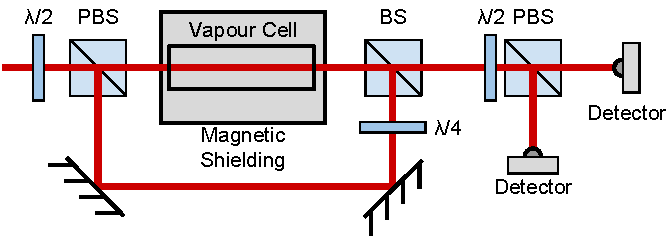
\includegraphics[width=\linewidth]{Figs/PolSpec.pdf}
    \captionof{figure}{A schematic of polarization spectroscopy with a balanced polarimeter. The power balance between the probe and pump beam is controlled with the leftmost $\lambda/2$ waveplate and \glsfirst*{pbs}. The $\lambda/4$ waveplate is adjusted to produce the circularly polarized pump beam. The non-polarizing 50:50 \gls*{bs} is used to make the beams colinear and counter-propagate through the atomic sample without altering the polarization of the circular pump or linear probe. The final $\lambda/2$ waveplate and \gls*{pbs} form the balanced polarimeter that monitors the polarization rotation of the probe.}
    \label{polspec_schematic}
\end{Figure}

A schematic diagram for \gls*{ps}\cite{wieman_doppler-free_1976, demtroder_laser_2014} is shown in figure \ref{polspec_schematic}. A circularly polarized pump beam from a monochromatic tunable laser induces frequency dependent, circular birefringence in an atomic gas sample by optical pumping. A linearly polarized beam from the same laser probes the birefringence by measuring the rotation of the probe's polarisation. To prevent Faraday rotation the atomic sample is shielded from external magnetic fields. A measurement of the probe's polarization rotation gives a frequency dependent error signal which can be used for laser locking to atomic transitions.

The polarization rotation of the probe is monitored using a balanced polarimeter consisting of a half-wave plate, \gls*{pbs} and two detectors. The difference signal from the two detectors provides a steep, background-free, antisymmetric, dispersion shaped error signal with a frequency width around 15\,MHz which is ideal for locking\cite{pearman_polarization_2002}.

Neglecting the birefringence of the windows of the atomic cell, the error signal for \gls*{ps} is given by the difference in intensity at the two detectors\cite{pearman_polarization_2002}:
\begin{align}
I_{PS} = I_x-I_y = -I_0 \cos(2\phi+2\Phi)\label{I_PS}
\end{align}
where $I_x,y$ are the horizontal and vertical linearly polarized components of the probe after the sample, $I_0$ is the intensity of the probe in the absence of a pump beam, $\phi$ is the angle of polarization of the probe in the absence of a pump beam and $\Phi$ is the additional rotation due to the birefringence induced by the pump. The largest \gls*{ps} spectrum is produced when $\phi=\pi/4$ and since $\Phi$ is small equation \ref{I_PS} can be approximated to
\begin{align}
I_{PS} \approx I_0 2\Phi.
\end{align}

If we define the difference in refractive indices for the $\sigma^\pm$ components of the probe, $n_\pm$, as $\Delta n = n_+ - n_-$ then we can write\cite{hecht_optics_1987}
\begin{align}
\Phi = \frac{\pi L \Delta n}{\lambda}
\end{align}
where $L$ is the length of the atomic sample and $\lambda$ is the wavelength.

The spectral profile of the difference in absorption coefficients for the atomic medium in the vicinity of a resonance is a Lorentzian with \gls*{fwhm} $\Gamma$\cite{demtroder_laser_2003}:
\begin{align}
\Delta \alpha = \frac{\Delta\alpha_0}{1+4\left(\frac{\delta}{\Gamma}\right)^2}.
\end{align}
Here, $\delta=\omega_L-\omega_A$ is the detuning of the laser from the resonance where $\omega_L$ is the angular frequency of the laser and $\omega_A$ the angular frequency of the atomic resonance. $\Delta\alpha_0$ is the difference in absorption coefficients for the $\sigma^\pm$ circular polarization components at $\delta=0$ and $\Gamma$ is the lifetime of the excited state of the resonance transition.

The refractive index and absorption coefficient of the medium can then be related through the Kramers-Kronig dispersion relation\cite{demtroder_laser_2003} to give
\begin{align}
\Delta n = \Delta\alpha_0 \frac{2c}{\omega_0 \Gamma}\frac{\delta}{1+4\left(\frac{\delta}{\Gamma}\right)^2}.\label{result}
\end{align}

$\Delta\alpha_0$ is given by the sum over all $m_F$ ground states of the difference in line-centre absorption for each circular polarization weighted by the ground ($F, m_F$) and excited state ($F', m_{F\pm1}$) population difference,
\begin{align}
\Delta\alpha_0 = \sum_{m_F=-F}^{+F} \alpha_{(F,m_F\rightarrow F',m_{F+1})}(P_{F,m_F}-P'_{F',m_{F+1}})\nonumber\\
-\alpha_{(F,m_F\rightarrow F',m_{F-1})}(P_{F,m_F}-P'_{F',m_{F-1}})
\end{align}

$\alpha_{(F, m_F\rightarrow F',m_{F\pm1})}=N \sigma(\omega)$ where $N$ is the number of interacting atoms and $\sigma(\omega)$ is the absorption cross section for the transition and $P_{F,m_F}$ refer to the populations of the various atomic states. The populations of an atomic ensemble do not evolve faster than the spontaneous transition rate $\tau=1/\Gamma$, therefore for timescales of order $\tau$, the populations can be considered to be constant. The absorption cross section is independent of the detuning of the probe so we can say that on short timescales that $\Delta\alpha_0$ is constant. For changes in laser frequency at this timescale equation \ref{result} still produces an ideal locking signal.

Laser frequency noise can extend to much higher frequencies than those at which the populations evolve, and thus the polarization spectroscopy signal of equation \ref{result} can provide a feedback bandwidth not limited by the usual absorption (spontaneous decay) bandwidth of $\Gamma/2$ (3\,MHz in the case of Rb).

\begin{Figure}
    \centering
    \captionsetup{type=figure}
    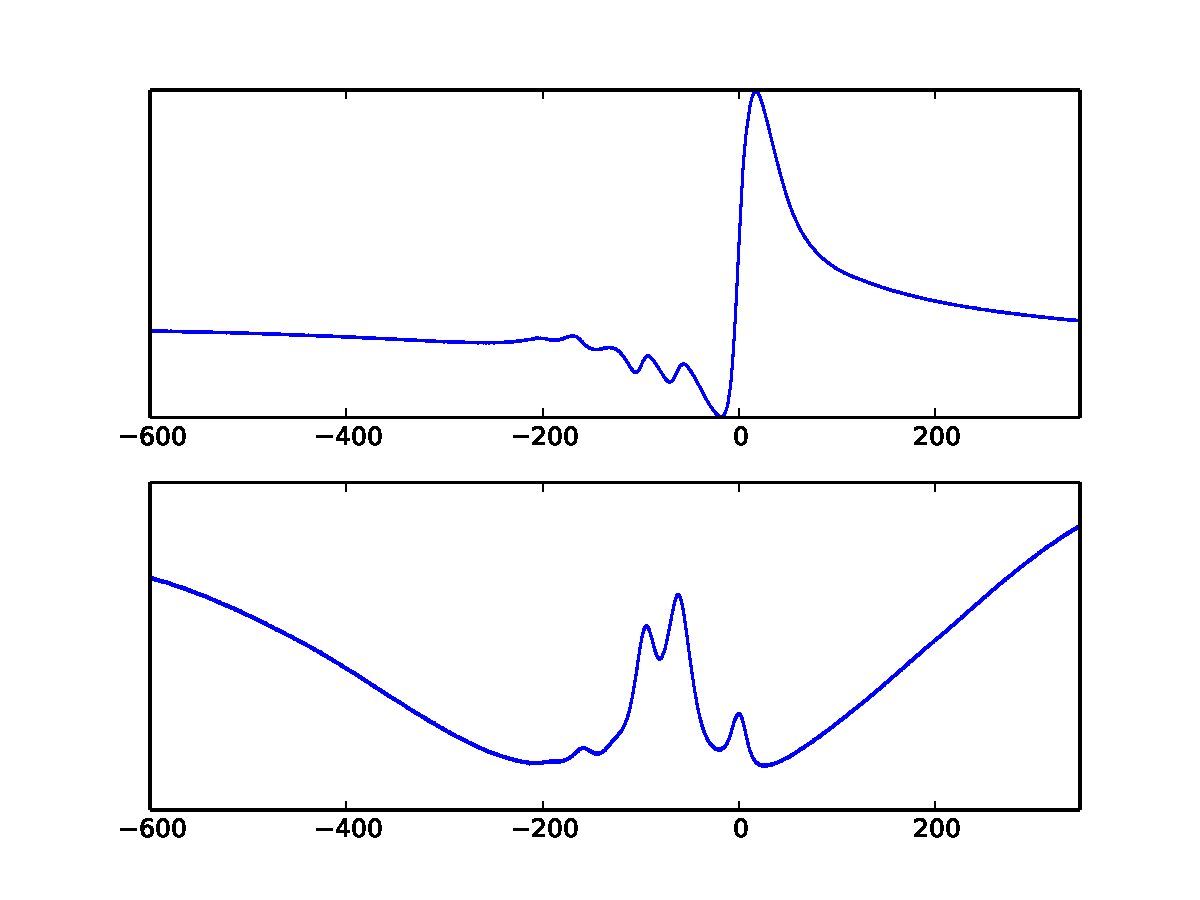
\includegraphics[width=\linewidth]{Figs/spectra.pdf}
    \captionof{figure}{An example of the polarization spectrum of the Rb$^{85}$ 5$^\text{2}$S$_\text{1/2}$ to 5$^\text{2}$P$_\text{3/2}$ transition. Label the various transitions too.{\color{red} WIP figure.}}
    \label{polspec_spectrum}
\end{Figure}

\section{Experiment}

Two separate Littrow configuration \glspl*{ecdl} were individually locked using \gls*{ps} and high bandwidth feedback. The lasers are controlled with commercial laser controllers\cite{mogbox} for temperature control, current supply and piezo control. 

Both laser beams were split by a \gls*{pbs} and the subsequent beams were then fibre coupled into polarization maintaining fibres. The output of the fibres led to the \gls*{ps} locking and the linewidth measurements as described in section \ref{results_section}.

The locking beams were polarized with Glan-Thompson prisms before entering the \gls*{ps} setup shown in figure \ref{polspec_schematic} in order to eliminate polarisation drift from the fibres. Telescopes were used to increase the width of the locking beams to fill the apertures of the magnetic shielding, to approximately 1\,cm diameter, allowing them to interact with more atoms thus increasing $|\Delta\alpha_0|$\cite{demtroder_laser_2003} and improving the \gls*{snr}.

The \gls*{ps} detectors were 100\,MHz bandwidth photodiodes\cite{tl_det} connected to 14\,MHz bandwidth servo controllers\cite{nf_servo}. The servo controllers generated the difference signal from the balanced polarimeter detector signals to produce the error signal and shaped the sero response. The output of the servo controllers was connected to the fast modulation inputs of the lasers. The lasers had fast current feedback that could eith be DC-coupled, with bandwidths of 40\,MHz\cite{dl_pro} and 10\,MHz\cite{mog_ecd003}, or AC-coupled, 100\,kHz\,\textendash\,40\,MHz\cite{dl_pro} and 10\,kHz\,\textendash\,10\,MHz\cite{mog_ecd003}.

The servo controllers could also provide the error signal to the laser controllers\cite{mogbox} which were able to modulate the piezo and current supply to aid the locking. The controller piezo feedback was limited by a bandwidth of 200\,Hz and the current feedback by a bandwidth of 50\,kHz.

\section{Results} \label{results_section}


{\color{red}Motivate linewidth measurements and bandwidth measurement. 3 different linewidth measurements to confirm performance. Bandwidth measurement for what?}

\subsection{Bandwidth}

The bandwidth of the locking system can be determined by examining the frequency spectrum of the error signal on and off the atomic resonance. The point at which these spectra cross indicates where the signal (on resonance) meets the noise (off resonance). This is shown in figure \ref{bandwidth}. The 0db noise limite bandwidth is 38\,MHz.

{\color{red}Something something Bode bumps/servo bumps.}

\begin{Figure}
    \centering
    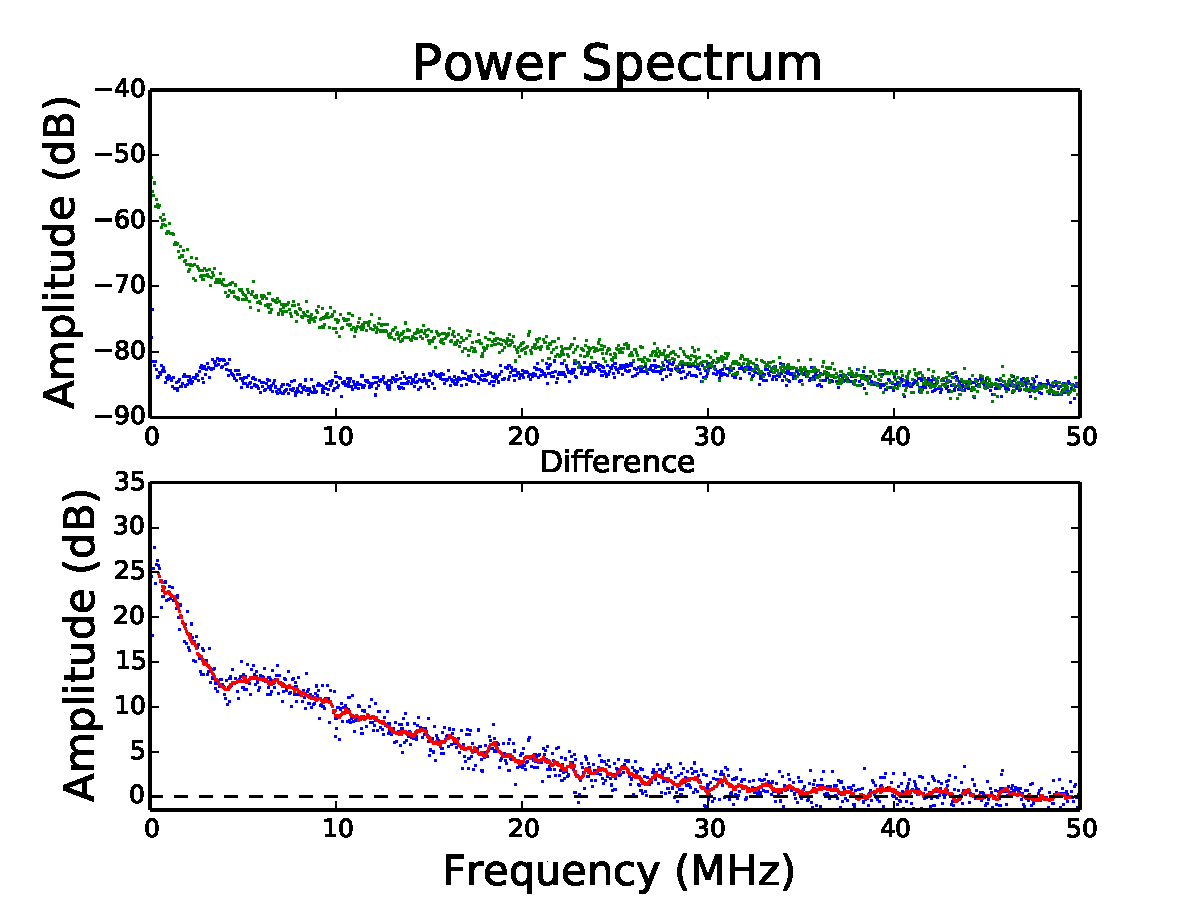
\includegraphics[width=\linewidth]{Figs/bandwidth.pdf}
    \captionsetup{type=figure}
    \captionof{figure}{Frequency bandwidth measurement of the polarization spectroscopy measurement. In the upper graph the green represents the frequency spectrum of the error signal while the laser is unlocked and centred on the Rb$^{85}$ 5$^\text{2}$S$_\text{1/2}$ to 5$^\text{2}$P$_\text{3/2}$ transition and the blue represents the same signal far from the transition. The lower graphs shows the difference between the on and off resonance spectra (blue) along with a 10 point moving average of the difference (red). {\color{red} This figure needs some pretty-fying. Linear or Log scale? Sat Abs for comparison?}}
    \label{bandwidth}
\end{Figure}

\subsection{Frequency Noise Measurements}
\begin{Figure}
    \centering
    \captionsetup{type=figure}
    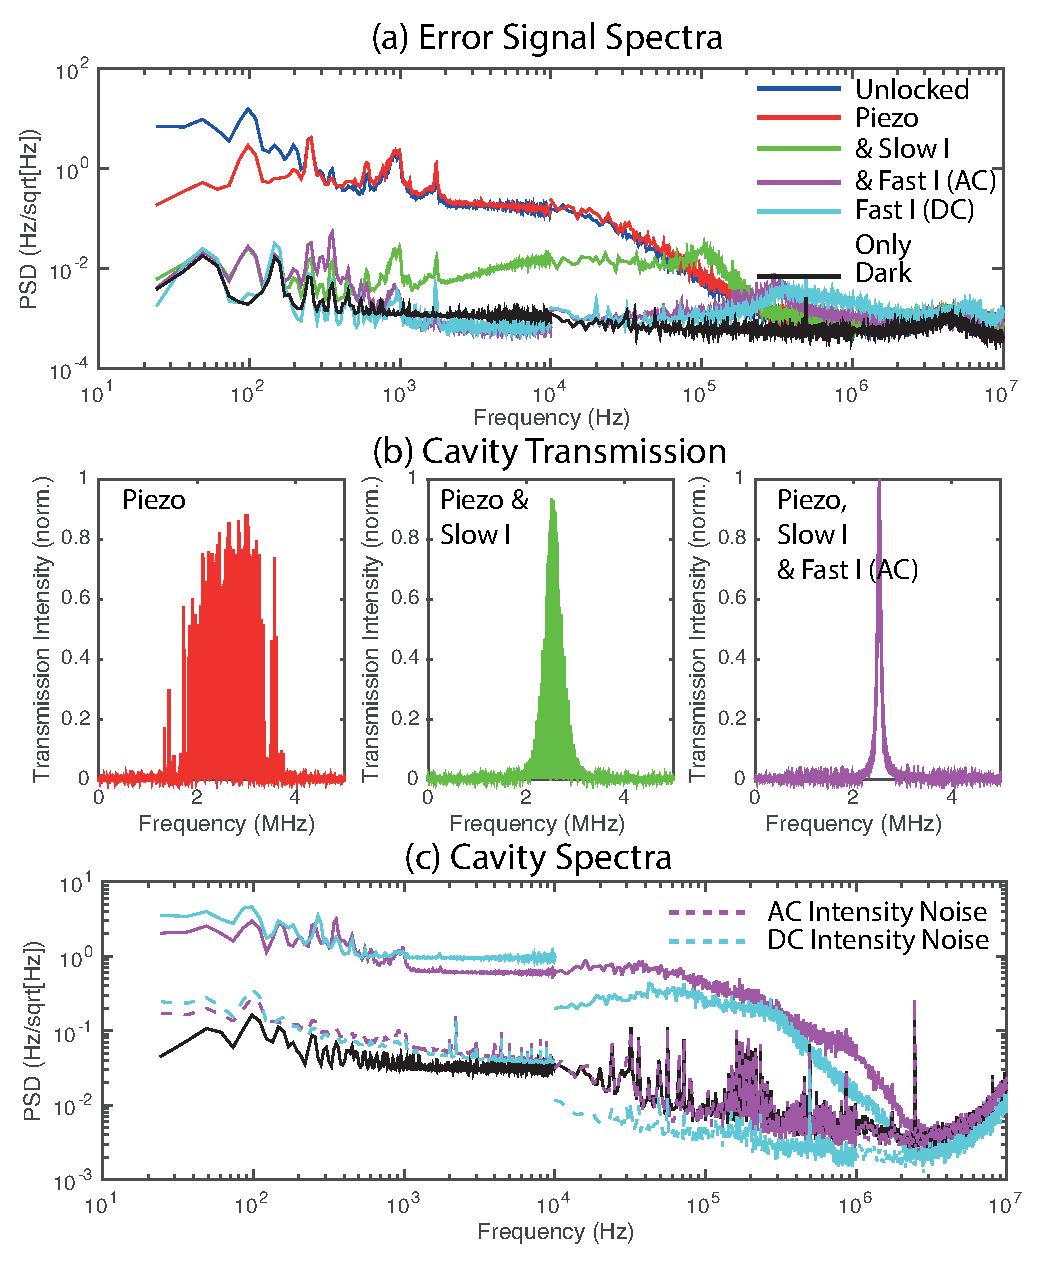
\includegraphics[width=\linewidth]{Figs/150904_SpectralDensityPlotsV102.eps}
    \caption{Frequency noise measurements. (a) \Gls*{lsd} {\color{red}(or is it PSD?)} measurements of polarization spectroscopy error signal frequency noise for a range of laser locking regimes: Piezo = piezo-only locking; Slow I = slow current feedback (40\,kHz bandwidth); Fast I = fast current feedback (maximum 14\,MHz bandwidth) either AC-coupled in combination with piezo and slow I feedback, or DC-coupled only. (b) Cavity transmission intensity as a function of AOM frequency. Cavity \gls*{fwhm} linewidth is 71.6\,kHz, scan time was 10\,ms. (c) \Gls*{lsd} measurements of transmitted cavity signal at half peak height for high-bandwidth locks. Also shown are the intensity noise of the laser, measured by removing the cavity and measuring frequency fluctuations with an intensity equal to half the peak transmission intensity. For (a) and (c) noise below $10^4$\,Hz was measured with a high dynamic range audio digitizer with a resolution bandwidth (RBW) of 12.2\,Hz; noise between $10^4$\textendash$10^6$\,Hz was measured with a spectrum analyzer with RBW of 30\,Hz, and measurements above $10^6$\,Hz were measured with a spectrum analyzer with a RBW of 300\,Hz.}
    \label{noise_measurement}
\end{Figure}

{\color{red} Remove the DC measurements from the figure and edit the discussion to suit.}


The frequency noise \gls*{lsd} (square-root of power spectral density) was determined with a high dynamic range audio digitizer (low frequency) and frequency radio spectrum analyzer (medium and high frequency). The spectrum analyzer was calibrated using the slope of the error signal and the known input impedance. The low frequency data was calibrated by matching to the spectrum analyzer data {\color{red}(at some frequency? Check with Ben.)}. Figure \ref{noise_measurement}(a) shows the noise spectra for a number of different cases, with AC and DC referring to the coupling of the error signal to the diode current. For the AC case, the piezo and low-bandwidth current feedback were also implemented. For the DC coupling, all feedback was supplied through the fast current modulation input only. The bandwidth of the locking increased, so did the reduction in noise, with the bandwidth of the piezo-only feedback being of order 200\,Hz, slow current feedback 70\,kHz, and fast locking 200\,kHz.\\

The measurement of noise on the error signal for the fast current feedback was limited by the noise floor of the measurement system, measured by blocking laser light on the detectors. Below 30\,kHz the signal noise was below the noise floor due {\color{red}to the suppression of noise within the feedback loop(?)}. A more sensitive and precise measure of the frequency spectra required a frequency discriminator. In this case we chose to use an ultra-stable optical cavity with a finesse of 20942, corresponding to a \gls*{fwhm} linewidth of 71.6\,kHz. The narrow linewidth of the cavity allowed us to measure noise up to 10\,MHz, limited by the bandwidth of the detector. Figure \ref{noise_measurement}(b) shows cavity transmission signals as the laser frequency is scanned with an AOM. The resulting traces provide a clear illustration of the effect of increased locking bandwidth: with piezo locking only the peak appears broad as the laser jitters around the resonant frequency. With slow current feedback, the peak becomes narrower and taller, and finally we see the effect of high-bandwidth feedback with a peak that has a \gls*{fwhm} limited by the cavity finesse, indicating a laser linewidth much smaller than the cavity linewidth.\\

By choosing a static \gls*{aom} frequency such that the transmitted laser intensity through the optical cavity is half the peak intensity, where the transmission-frequency response is approximately linear, we can analyze the frequency noise of the laser through the cavity transmission signal. This is shown in figure \ref{noise_measurement}(c) for fast AC and DC locking, both now well above the noise floor. The other locks shown in figure \ref{noise_measurement}(a) could not be evaluated using this method, as they were too noisy to stay within the linear frequency response range of the cavity. The AC and DC coupled suppression is flat at low frequencies, reducing above 50\,kHz. The peaks in the noise floor between $10^4$ and $10^6$\,Hz are due to electromagnetic interference on the detector. A drawback of noise measurements with a cavity is that laser intensity noise is mapped into frequency noise. To examine the intensity noise spectrum the detector was placed in front of the cavity with the same laser intensity incident on it as that used for the linewidth measurement. This is shown in figure \ref{noise_measurement}(c). The intensity noise is well below the cavity transmission noise and we can therefore assume that the measured spectrum is dominated by the frequency fluctuations of the laser.\\

We can extract a linewidth for the laser from the cavity data using two methods: first we can map the intensity noise of the transmitted, locked cavity signal to the cavity transmission frequency response. The distribution of frequencies can then be fitted with a Gaussian to determine the \gls*{fwhm} linewidth of the laser. For our system this gives a linewidth of 5.42\,kHz. Unfortunately this method is also sensitive to the laser intensity noise which is mapped to frequency noise in the analysis. To illustrate this, calculating a laser ``linewidth'' from the intensity noise alone gives a ``linewidth'' of 3.26\,kHz, suggesting that the real laser linewidth is well below the measured 5.42\,kHz. To extract an exact linewidth with this method, a cavity with a higher finesse combined with intensity stabilization could be used. The second method involves integrating the power spectral density to determine the RMS linewidth\cite{negnevitsky_wideband_2013}. For the AC lock this gives an RMS linewidth of 350\,Hz. Assuming the linewidth has a Gaussian shape gives a FWHM linewidth of approximately 850\,Hz, much lower than that calculated using the above method. The results from these methods are summarized in Table \ref{linewidth_table}.\\

\begin{Figure}
\centering
\begin{tabular}{|c|c|}
\hline
  Method & Linewidth (kHz) \\ \hline
  (i) Map Lorentzian (signal)  & 5.42 \\
  (ii) Map Lorentzian (noise) & 3.26 \\
  (iii) PSD Integral & 0.85 \\
  (iv) Heterodyne & 1.4 \\ \hline\end{tabular}
\captionsetup{type=table}
\caption{Linewidth results. Mapping the transmission signal through a cavity with a \gls*{fwhm} of 71.6\,kHz to a Lorentzian signal [(i) and (ii)] is limited by the laser intensity noise. The results from integrating the power-spectral density signal (Fig.~\ref{noise_measurement}) and the heterodyne beat-note (Fig.~\ref{beatnote}) both give a value for the linewidth of less than 1\,kHz. {\color{red}Errors would be nice.}}
\label{linewidth_table}
\end{Figure}

\subsection{Heterodyne Measurements}
The heterodyne measurements were made by frequency shifting one of the laser beams with an \gls*{aom} and combining the two beams to be colinear and coincident onto a 1\,GHz bandwidth detector\cite{nf_det}. The output of this detector is measured with a radio frquency spectrum analyzer\cite{rs_sa}.

A typical heterodyne measurement of the signal produced by the two lasers is shown figure \ref{beatnote}. The Gaussian \gls*{fwhm} width of the beatnote shown is 2.0\,kHz. If Gaussian linewidths and identical lasers are assumed then there is a factor of $\sqrt{2}$ between the beatnote \gls*{fwhm} and the laser linewidth \gls*{fwhm} which corresponds to a laser \gls*{fwhm} linewidth of 1.4\,kHz.

{\color{red}Discuss beatnote shape. Shoulders, sidebands, central peak. The sidebands of the beatnote are located at $\pm$360\,kHz. This looks useful.\cite{di_domenico_simple_2010} The sidebands indicate the effective servo bandwidth.}

Diagnostic measurements performed with the high-finesse cavity indicated that the frequency jitter of one of the laser setups was significantly larger than that of the other. Unfortunately the source of the jitter is difficult to determine. If we estimate that the spectral linewidth of the `jittery' laser was double that of the other then the linewidth of the more stable laser would be 1.15\,kHz.

\begin{Figure}
    \centering
    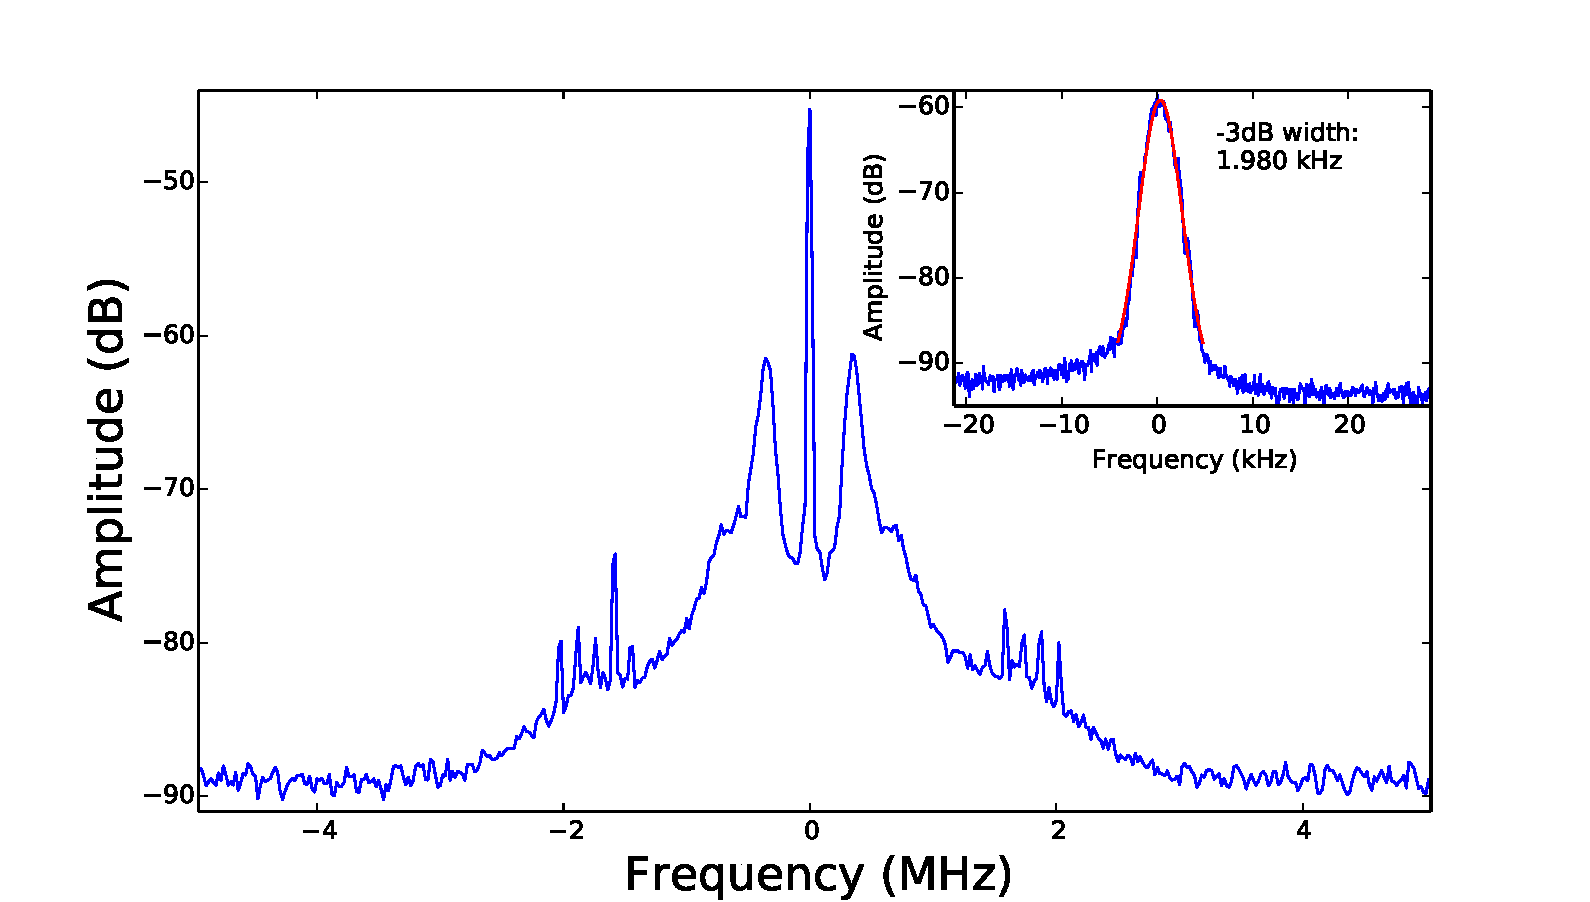
\includegraphics[width=\linewidth]{Figs/beatnote_inset.pdf}
    \captionsetup{type=figure}
    \captionof{figure}{Typical heterodyne beatnote for the two lasers locked with \gls*{ps}. The figure and inset figure are both 50 shot averages with resolution bandwidths of 30\,kHz and 100\,Hz and total measurement times of approximately 0.5\,s and 2\,s respectively.}
    \label{beatnote}
\end{Figure}

\section{Conclusion}

The spectral linewidth achievable with \gls*{ps} is demonstrably lower than previously indicated. The \gls*{snr} of the locking system is the current limiting factor of the linewidth reduction. Reducing the electronic noise in the system and increasing the number of intereacting atoms with wider beams, longer gas cells or heated gas cells could help reduce the linewidth further. The current experimental setup is an example of a low cost, low linewidth and simple laser source frequency stabilized to an atomic reference.

{\color{red}Drift?}

\section{Acknowledgements}
\begin{itemize}
\item Funding sources.
\item Alex for electronics help (or should he be an author?)
\item Rory for sanity checking of code.
\item Andre Luiten for equipment and advice
\end{itemize}

\bibliographystyle{plain}
\bibliography{Library,Equipment}

\end{multicols}
\end{document}
